\documentclass[aps,prb,twocolumn,floatfix,nofootinbib,superscriptaddress]{revtex4-2}
\usepackage{amsmath,amssymb,mathtools,bm}
\usepackage{booktabs}
\usepackage{graphicx}
\usepackage[colorlinks=true,linkcolor=blue,citecolor=blue,urlcolor=blue]{hyperref}
\usepackage{microtype}

\graphicspath{
  {../results/N20x24_state_projector_pump_s100_v1/analysis/figures/}
  {../results/N20x24_state_projector_pump_s100_v1/analysis/crossing_diagnostics_v1/}
}

\newcommand{\tr}{\operatorname{tr}}
\newcommand{\ii}{\mathrm{i}}

\begin{document}

\title{Trajectory-Resolved Spectral Flow of Monitored Domain-Wall States}
\author{Asadullah Bhuiyan}
\affiliation{Class-A fermionic adaptive-circuit project}
\date{September 10, 2026}

\begin{abstract}
We study a static spectral-flow diagnostic of pure Gaussian states prepared by
the monitored class-A circuit.  Each trajectory supplies an occupied
projector, from which we construct a spectrally flattened one-particle parent
and thread one transverse flux quantum.  A previous-projector-overlap rule
defines the continued occupied subspace.  For $N_x\times N_y=20\times24$ and
$n_{\mathrm{shell}}=1$, the 64-interval continuation produces a sharply bimodal
response: 71 of 100 soft-wall states and 36 of 100 hard-wall states transfer
nearly one unit of charge, while the remaining states close at zero.  The raw
mean endpoints are $(+0.70740,-0.70716)$ for the soft wall and
$(+0.35937,-0.35940)$ for the hard wall under counterclockwise and clockwise
threading, respectively.  The same endpoint projectors yield 64 and 30 unit
events on a 128-interval grid.  An independent $24\times24$ ensemble gives 91
soft-wall and 46 hard-wall events on the 64-interval grid.  These results
establish trajectory-resolved wall spectral flow, but they also show that the
global overlap selector is sensitive to how a finite-width avoided crossing is
resolved.  The binary response is therefore a property of the specified
continuation protocol, not by itself a grid-converged topological index or a
real-time monitored pump.
\end{abstract}

\maketitle

\section{The question being asked}

The monitored circuit prepares a pure Gaussian state rather than a ground
state of a microscopic Hamiltonian.  The question here is deliberately
narrow: after one trajectory has prepared such a state, does its occupied
one-particle subspace carry the same wall-to-wall spectral flow as a Chern
insulator under flux insertion?

This question separates naturally into two parts.  The first is the state
prepared by the circuit.  The second is the rule used to continue that state
through flux.  The charge observable is simple once this path has been fixed;
the subtlety lies in defining the path.  In particular, the calculation below
does not evolve the monitored circuit while the flux changes.  It constructs a
static family of trajectory-dependent flattened parents and continues an
occupied spectral subspace through that family.

The distinction matters.  A nonzero endpoint response in this calculation is
evidence for spectral flow of the prepared projector.  It is not an unbiased
Born-ensemble current, and it is not a claim that a particle was observed to
cross the sample during monitored time evolution.

\section{Monitored endpoint ensemble}

For each wall construction and each sample $s=0,\ldots,99$, the canonical CPU
entry point \texttt{classA\_U1FGTN.run\_markov\_circuit} generates an
independent trajectory.  The primary ensemble uses
\begin{align}
 (N_x,N_y)&=(20,24), & T&=2N_y=48,\\
 n_{\mathrm{shell}}&=1, & (\alpha_1,\alpha_2)&=(1,30).
\end{align}
The initial state is a random pure Gaussian state at half filling.  The
overcomplete-Wannier (OW) measurements are applied in raster-$y$ order with
perfect correction, no postselection, and complex128 arithmetic.  The two
walls lie at $x=5$ and $x=15$.  The soft construction retains the full spatial
mass profile, whereas the hard construction terminates OW support at the
active slab.

One complete monitored trajectory is the independent sampling unit.  The
deterministic seed is derived from root seed $2026090304$, the wall type, and
the sample index.  Soft- and hard-wall trajectories are independent rather
than paired.  Perfect feedback correction preserves the intended circuit
rule, but it need not preserve the particle number of an individual Born
trajectory.  We therefore retain the final occupied rank $r_\xi$ of every
trajectory $\xi$ instead of projecting all samples back to a common rank.

\section{From an occupied frame to a threaded parent}

Let
\begin{equation}
 F_\xi\in\mathbb C^{2N_xN_y\times r_\xi},\qquad
 F_\xi^\dagger F_\xi=\mathbf{1}_{r_\xi},
\end{equation}
be an occupied frame for trajectory $\xi$.  Its columns are a basis, not
additional physical degrees of freedom.  The basis-independent object is the
one-particle correlation projector
\begin{equation}
 G_\xi=F_\xi F_\xi^\dagger,
 \qquad G_\xi^2=G_\xi=G_\xi^\dagger .
 \label{eq:projector}
\end{equation}
The implementation historically stores this matrix under the name \texttt{C};
we use $G$ here to retain the notation of the main technical work.

We associate to this projector the flattened one-particle parent
\begin{equation}
 h_\xi(0)=\mathbf{1}_{2N_xN_y}-2G_\xi .
 \label{eq:parent}
\end{equation}
The occupied and empty subspaces of $G_\xi$ are then the $-1$ and $+1$
eigenspaces of $h_\xi(0)$.  Equation~\eqref{eq:parent} introduces no new
state: $G_\xi=(\mathbf{1}-h_\xi)/2$.  Its purpose is to turn occupation into
spectral ordering.  Once this is done, twisting the parent supplies both the
occupied and empty instantaneous eigenspaces needed to define a spectral
continuation.  The parent is trajectory specific and should not be confused
with the microscopic controller Hamiltonian used during preparation.

The periodic direction is $y$.  For one-particle labels
$a=(x,y,\mu)$ and $b=(x',y',\mu')$, let $d_y(a,b)$ denote the minimum-image
displacement on the $N_y$-site ring.  In the uniform gauge we define
\begin{align}
 \widetilde h_{\xi,ab}(\phi)
 &=h_{\xi,ab}(0)
   \exp\!\left[\frac{\ii\phi}{N_y}d_y(a,b)\right],\\
 h_\xi(\phi)&=\frac12\left[\widetilde h_\xi(\phi)
                    +\widetilde h_\xi^\dagger(\phi)\right].
 \label{eq:threaded-parent}
\end{align}
The second line removes only floating-point anti-Hermiticity.  It does not
modify the intended flux family.

Clockwise (CW) and counterclockwise (CCW) paths use
\begin{equation}
 \phi_j^{(\sigma)}=-\sigma\epsilon
 +\sigma\frac{2\pi j}{M},
 \qquad \epsilon=10^{-7},\quad \sigma=\pm1,
 \label{eq:grid}
\end{equation}
with $j=0,\ldots,M$.  The signed offset chooses a one-sided representative at
the seam where an exact crossing would otherwise make the initial label
ambiguous.  It is not a physical flux ramp and cannot manufacture an integer
response.

\section{Previous-projector continuation}

At flux point $j$, diagonalize
\begin{equation}
 h_\xi(\phi_j)u_{a,j}=E_{a,j}u_{a,j}.
\end{equation}
Suppose $P_{j-1}$ is the rank-$r_\xi$ projector selected at the preceding
point.  The weight
\begin{equation}
 \omega_{a,j}
 =\langle u_{a,j}|P_{j-1}|u_{a,j}\rangle
 =\|F_{j-1}^\dagger u_{a,j}\|^2
 \label{eq:weight}
\end{equation}
measures how much of the new eigenvector already lies in the previously
occupied subspace.  We select the $r_\xi$ eigenvectors with the largest
$\omega_{a,j}$ and define
\begin{equation}
 P_j=\sum_{a\in\mathcal I_j}|u_{a,j}\rangle\langle u_{a,j}|.
 \label{eq:selector}
\end{equation}
Instantaneous energy enters only as a deterministic tie breaker.

This prescription can be stated without choosing a frame.  Among projectors
formed from $r_\xi$ eigenvectors of $h_\xi(\phi_j)$, Eq.~\eqref{eq:selector}
maximizes
\begin{equation}
 \tr(P_{j-1}P_j)=\sum_{a\in\mathcal I_j}\omega_{a,j}.
\end{equation}
The computed path is therefore a path of projectors.  A frame is retained only
as a numerically efficient representation of that path; arbitrary unitary
rotations among its occupied columns do not change the result.

As a control, we also form the instantaneous projector $P_j^{\mathrm{inst}}$ from
the $r_\xi$ lowest eigenvalues independently at every flux.  It closes after
one flux quantum.  The distinction between $P_j$ and $P_j^{\mathrm{inst}}$ is thus
not the final Hamiltonian---the two paths end at gauge-equivalent spectral
problems---but the occupation labels carried through the crossing.

\section{Subsystem charge}

Let $R_L$ and $R_R$ project onto the left and right half cylinders,
respectively.  For $N_x=20$,
\begin{align}
 R_L&=\sum_{x=0}^{9}\sum_{y,\mu}|x,y,\mu\rangle\langle x,y,\mu|,\\
 R_R&=\sum_{x=10}^{19}\sum_{y,\mu}|x,y,\mu\rangle\langle x,y,\mu|.
\end{align}
The continued regional charges and their changes from the starting projector
are
\begin{align}
 N_A(\phi_j)&=\tr(R_AP_j),\\
 \Delta N_A(\phi_j)&=N_A(\phi_j)-\tr(R_AP_0),
 \qquad A=L,R .
\end{align}
The transverse transfer is
\begin{equation}
 q_x(\phi_j)=\frac{\Delta N_R(\phi_j)-\Delta N_L(\phi_j)}{2}.
 \label{eq:qx}
\end{equation}
Because the rank is fixed and $R_L+R_R=\mathbf{1}$,
$\Delta N_L+\Delta N_R=0$ up to roundoff.  Hence
$q_x=\Delta N_R=-\Delta N_L$.  An endpoint $q_x\simeq+1$ is simply one unit
removed from the left half and added to the right half in the continued
projector.  The reverse process gives $q_x\simeq-1$.

We report raw CW and CCW values separately.  The paired combination
\begin{equation}
 q_x^{\mathrm{odd}}=\frac{q_x^{\mathrm{CCW}}-q_x^{\mathrm{CW}}}{2}
 \label{eq:qodd}
\end{equation}
is used only as a compact measure of direction reversal and to reproduce the
original event ledger.  It is not substituted for the sample-resolved raw
distribution.

\section{The 64-interval result}

All 200 monitored endpoints and all 400 directional continuations completed
for the $20\times24$, $n_{\mathrm{shell}}=1$ ensemble.  An independent readback
audit verified every result/completion pair, comprising 1.331~GiB of output.
The raw endpoint means and sample standard deviations are
\begin{align}
 \overline{q_x^{\mathrm{CCW}}}_{\mathrm{soft}}&=+0.70740,
 &s_{\mathrm{soft}}^{\mathrm{CCW}}&=0.45442,\\
 \overline{q_x^{\mathrm{CW}}}_{\mathrm{soft}}&=-0.70716,
 &s_{\mathrm{soft}}^{\mathrm{CW}}&=0.45428,\\
 \overline{q_x^{\mathrm{CCW}}}_{\mathrm{hard}}&=+0.35937,
 &s_{\mathrm{hard}}^{\mathrm{CCW}}&=0.48157,\\
 \overline{q_x^{\mathrm{CW}}}_{\mathrm{hard}}&=-0.35940,
 &s_{\mathrm{hard}}^{\mathrm{CW}}&=0.48161.
\end{align}
The reversal is nearly exact: the largest samplewise direction-even endpoint
is $6.31\times10^{-3}$ for the soft wall and $1.68\times10^{-3}$ for the hard
wall.

The ensemble means hide the structure of the result.  On the $M=64$ grid,
71 soft-wall trajectories have $|q_x^{\mathrm{odd}}|>0.5$.  Their conditional mean
is $0.99617$ and their minimum is $0.95733$; every other soft-wall endpoint has
magnitude below $1.60\times10^{-8}$.  The hard-wall ensemble contains 36 such
events, with conditional mean $0.99828$ and minimum $0.98828$; every remaining
hard-wall endpoint again closes below $1.60\times10^{-8}$.  The response is
therefore a mixture of two trajectory-resolved sectors, not a fractional
charge attached to a typical state.

\begin{figure*}[t]
 \centering
 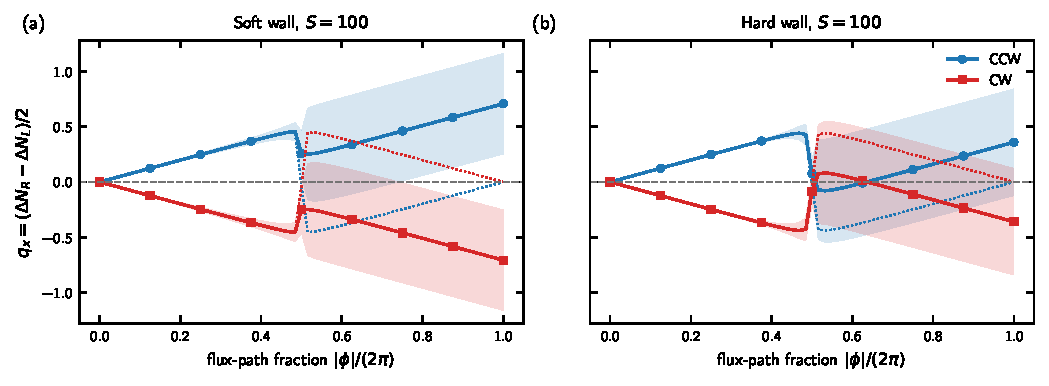
\includegraphics[width=\textwidth]{state_projector_pump_mean_qx.pdf}
 \caption{Static projector response at $N_x\times N_y=20\times24$,
 $n_{\mathrm{shell}}=1$, and $M=64$.  Each wall uses $S=100$ independent
 monitored trajectories prepared from random pure half-filled states for
 $T=48$ raster-$y$ cycles.  Curves are trajectory means and bands are one
 sample standard deviation.  Solid curves show the previous-projector
 continuation; dotted curves show independently refilled instantaneous
 projectors.  CW and CCW reverse the continued response, whereas the
 instantaneous control closes after one flux quantum.}
 \label{fig:mean-response}
\end{figure*}

\begin{figure*}[t]
 \centering
 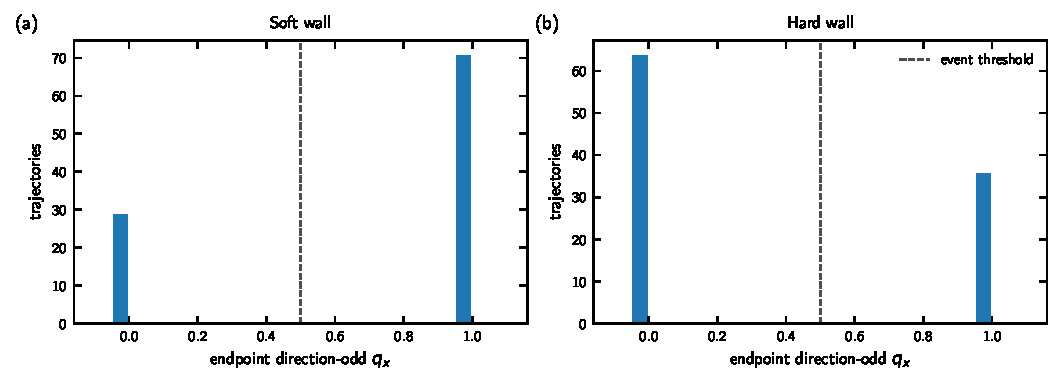
\includegraphics[width=\textwidth]{state_projector_pump_endpoint_histogram.pdf}
 \caption{Sample-resolved endpoint distribution for the same $S=100$
 ensembles.  The plotted direction-odd coordinate only superposes the paired
 CW and CCW reversals; the archived table retains both raw endpoints.  The
 dashed line at $0.5$ defines the descriptive event count.  It is not an
 acceptance threshold for topology or quantization.}
 \label{fig:endpoints}
\end{figure*}

The numerical residuals are far below either sector.  Across all 400 paths,
the largest violation of $\Delta N_L+\Delta N_R=0$ is
$2.84\times10^{-13}$, the largest instantaneous endpoint is
$1.59\times10^{-8}$, and the largest large-gauge parent mismatch is
$7.11\times10^{-16}$.  Final particle-number rank has negligible linear
association with the response (Pearson $-0.073$ for the soft wall and $0.020$
for the hard wall).  The zero/unit split is therefore not produced by charge
nonconservation or by the raw variation of final rank.

\section{What controls the binary sector}

Let $E_{1,j}\le\cdots\le E_{2N_xN_y,j}$ be the eigenvalues of the threaded
parent and let $r_\xi$ be the occupied rank.  The spectral pair at the
occupation boundary has gap
\begin{equation}
 \delta_{\mathrm{edge}}(\phi_j)
 =E_{r_\xi+1,j}-E_{r_\xi,j}.
 \label{eq:edge-gap}
\end{equation}
For every $20\times24$ trajectory, the minimum occurs at
$|\phi|\simeq\pi$.  Unit-transfer trajectories have systematically smaller
minimum gaps.  The soft-wall medians are $0.00611$ in the unit sector and
$0.02652$ in the closing sector; the hard-wall medians are $0.00673$ and
$0.02624$.  Using small gap as a descriptive classifier gives areas under the
receiver-operating curve of $0.898$ and $0.911$, respectively.  This is a
strong association, but not yet a proof of a topological dichotomy.

\begin{figure*}[t]
 \centering
 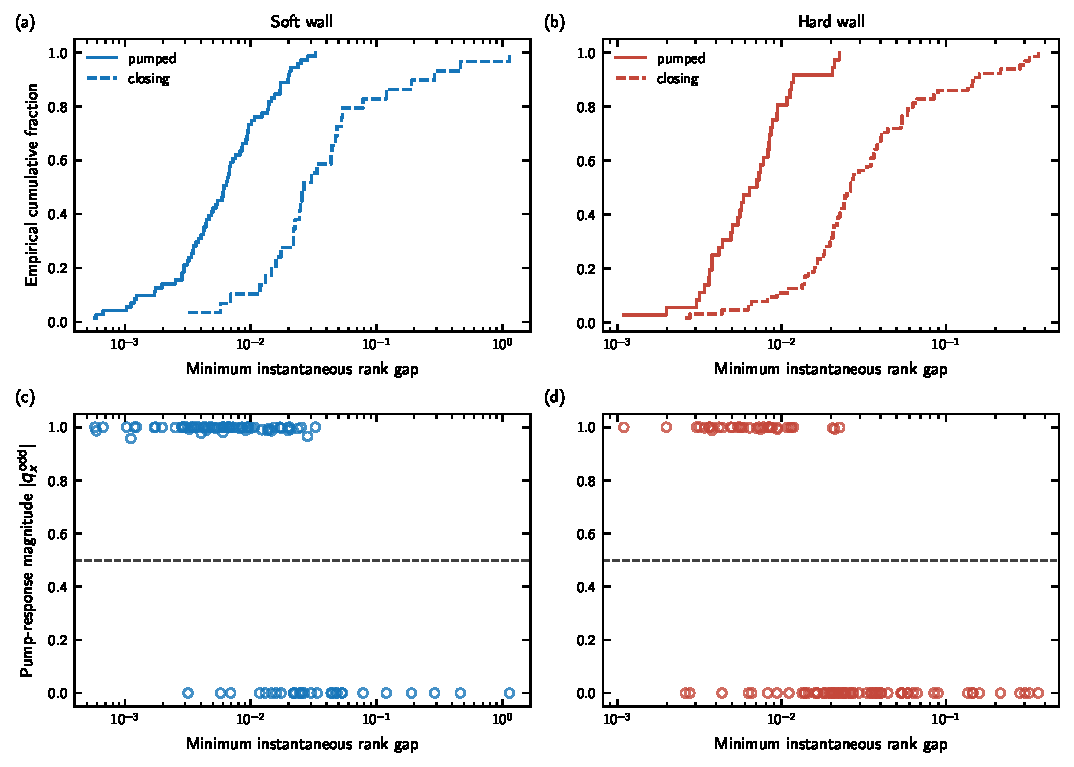
\includegraphics[width=0.82\textwidth]{ny24_pump_sector_vs_pi_crossing_gap.pdf}
 \caption{Relation between the $M=64$ endpoint sector and the minimum
 occupied--empty gap near $|\phi|=\pi$ for $S=100$ independent trajectories
 per wall.  The unit-transfer sector is concentrated at smaller gaps.  This
 diagnostic cannot by itself distinguish an intrinsic crossing from a
 finite-grid branch-selection effect.}
 \label{fig:crossing-gap}
\end{figure*}

The latter distinction is resolved by repeating the continuation on the
\emph{same} endpoint projectors with $M=128$.  Seven soft-wall samples and six
hard-wall samples move from the unit sector at $M=64$ to the closing sector at
$M=128$; no sample moves in the opposite direction.  The event counts become
64/100 and 30/100.  The corresponding raw endpoint means are
$(+0.63777,-0.63750)$ for the soft wall and
$(+0.29951,-0.29953)$ for the hard wall.

This is not ordinary quadrature error in Eq.~\eqref{eq:qx}.  The finite grid is
part of the continuation rule.  Near an avoided crossing, the eigenvectors
rotate over a flux scale set by the inter-wall hybridization.  A step larger
than that scale follows the same wall character across the exchange of energy
ordering; a sufficiently fine step follows the smooth finite-size energy
eigenprojector, which closes.  The $M=64$ binary distribution is therefore an
exact result for the stated overlap protocol, but it is not invariant under
refinement of that protocol.

\section{First transverse-width comparison}

An independent $N_x\times N_y=24\times24$ ensemble repeats the $M=64$ protocol
with $S=100$ trajectories per wall, $n_{\mathrm{shell}}=1$, $T=48$, and walls at
$x=6$ and $x=18$.  Table~\ref{tab:comparison} collects the directly comparable
raw endpoint means and unit-event counts.

\begin{table*}[t]
 \caption{Completed overlap-continuation ensembles.  Each row contains
 $S=100$ independent monitored trajectories per wall.  The event column uses
 the historical descriptive criterion $|q_x^{\mathrm{odd}}|>0.5$; the primary
 observables are the separate raw CW and CCW endpoints.}
 \label{tab:comparison}
 \begin{ruledtabular}
 \begin{tabular}{cccccccc}
 $N_x\times N_y$ & $M$ &
 $\overline{q_x^{\mathrm{CCW}}}$ soft & $\overline{q_x^{\mathrm{CW}}}$ soft & soft events &
 $\overline{q_x^{\mathrm{CCW}}}$ hard & $\overline{q_x^{\mathrm{CW}}}$ hard & hard events\\
 \hline
 $20\times24$ & 64  & $+0.70740$ & $-0.70716$ & $71/100$ & $+0.35937$ & $-0.35940$ & $36/100$\\
 $20\times24$ & 128 & $+0.63777$ & $-0.63750$ & $64/100$ & $+0.29951$ & $-0.29953$ & $30/100$\\
 $24\times24$ & 64  & $+0.90749$ & $-0.90726$ & $91/100$ & $+0.45896$ & $-0.45903$ & $46/100$
 \end{tabular}
 \end{ruledtabular}
\end{table*}

At fixed $M=64$, increasing the wall separation from 10 to 12 sites raises
the soft-wall event fraction by 0.20 and the hard-wall fraction by 0.10.  The
closing-sector median gap rises from $0.02652$ to $0.03367$ in the soft
ensemble and from $0.02624$ to $0.04019$ in the hard ensemble.  The
unit-sector medians at
$24\times24$ are $0.00740$ for both walls, while the closing-sector medians are
$0.03367$ and $0.04019$.

The width comparison is suggestive but not yet a scaling law.  The two sizes
use independent monitored ensembles, only two values of $N_x$ are complete,
and the global overlap rule itself changes under grid refinement.  The soft
increase is large; the hard increase is smaller and statistically compatible
with a broad range of width effects.  No thermodynamic limit should be inferred
from these two points.

\section{Interpretation}

The calculation has isolated a precise object.  A monitored trajectory
produces $G_\xi$.  The flattened parent $h_\xi=\mathbf{1}-2G_\xi$ promotes its
occupied/empty decomposition to a spectral problem.  The overlap selector
then carries an occupation label through the threaded spectrum, and $q_x$
reads the resulting left--right redistribution.  Once the path is specified,
there is no ambiguity in the charge measurement.

What is not fixed by $q_x$ is the branch through the finite-width wall
crossing.  The exact translation-invariant flattened-Hamiltonian benchmark
retains a clean wall crossing and gives $|q_x|=0.981$--$1.000$ under refined
continuation.  A trajectory-derived parent breaks transverse translation
symmetry and generically opens a sample-dependent avoided gap.  The global
$M=64$ overlap rule often crosses this gap diabatically, producing one unit of
wall transfer.  Refining the grid resolves some of the same gaps and instead
follows the smooth finite-size projector back to itself.

This exposes a noncommuting order of limits.  The inter-wall gap falls with
wall separation, whereas the edge-to-bulk separation remains finite.  The
spectral-flow limit is adiabatic relative to the bulk but diabatic relative to
the exponentially small inter-wall splitting.  Full finite-size adiabatic
continuation takes the opposite limit and closes.  A robust continuation must
therefore identify the isolated two-wall subspace and preserve wall character
inside it, rather than obtain the desired branch accidentally from a coarse
global grid.  That wall-diabatized calculation is documented separately and
should be regarded as the controlled successor to the present protocol.

The completed result supports three statements and no stronger ones.  First,
the prepared trajectory projectors retain wall-localized spectral structure.
Second, the specified $M=64$ overlap continuation produces sharply quantized
samplewise transfer with nearly exact CW--CCW reversal.  Third, the fraction of
such events depends on the avoided-crossing scale, the flux mesh, and probably
the transverse wall separation.  It does not establish a quantized response of
the trajectory-averaged state, a quantized monitored-time pump, or a universal
finite-width event probability.

\section{Reproducibility}

The $20\times24$, $M=64$ campaign is archived under
\path{results/N20x24_state_projector_pump_s100_v1}; its locked configuration
SHA-256 begins \texttt{aafda9bcd52995b48}.  The exact same endpoints at
$M=128$ are under
\path{results/N20x24_state_projector_pump_grid128_s100_v1}.  The independent
$24\times24$, $M=64$ ensemble is under
\path{results/N24x24_state_projector_pump_s100_v1}.  Each trajectory
and each directional continuation is stored as an atomic NPZ/result pair with
a checksum-bearing completion JSON.  The CSV tables retain wall type, sample
identity, final rank, and separate raw CW and CCW endpoints.  The crossing-gap
analysis is stored below the primary $20\times24$ analysis directory in
\path{crossing_diagnostics_v1}.

\end{document}
